\documentclass[a4paper,
fontsize=11pt,
%headings=small,
oneside,
numbers=noperiodatend,
parskip=half-,
bibliography=totoc,
final
]{scrartcl}

\usepackage[babel]{csquotes}
\usepackage{synttree}
\usepackage{graphicx}
\setkeys{Gin}{width=.4\textwidth} %default pics size

\graphicspath{{./plots/}}
\usepackage[ngerman]{babel}
\usepackage[T1]{fontenc}
%\usepackage{amsmath}
\usepackage[utf8x]{inputenc}
\usepackage [hyphens]{url}
\usepackage{booktabs} 
\usepackage[left=2.4cm,right=2.4cm,top=2.3cm,bottom=2cm,includeheadfoot]{geometry}
\usepackage{eurosym}
\usepackage{multirow}
\usepackage[ngerman]{varioref}
\setcapindent{1em}
\renewcommand{\labelitemi}{--}
\usepackage{paralist}
\usepackage{pdfpages}
\usepackage{lscape}
\usepackage{float}
\usepackage{acronym}
\usepackage{eurosym}
\usepackage{longtable,lscape}
\usepackage{mathpazo}
\usepackage[normalem]{ulem} %emphasize weiterhin kursiv
\usepackage[flushmargin,ragged]{footmisc} % left align footnote
\usepackage{ccicons} 
\setcapindent{0pt} % no indentation in captions

%%%% fancy LIBREAS URL color 
\usepackage{xcolor}
\definecolor{libreas}{RGB}{112,0,0}

\usepackage{listings}

\urlstyle{same}  % don't use monospace font for urls

\usepackage[fleqn]{amsmath}

%adjust fontsize for part

\usepackage{sectsty}
\partfont{\large}

%Das BibTeX-Zeichen mit \BibTeX setzen:
\def\symbol#1{\char #1\relax}
\def\bsl{{\tt\symbol{'134}}}
\def\BibTeX{{\rm B\kern-.05em{\sc i\kern-.025em b}\kern-.08em
    T\kern-.1667em\lower.7ex\hbox{E}\kern-.125emX}}

\usepackage{fancyhdr}
\fancyhf{}
\pagestyle{fancyplain}
\fancyhead[R]{\thepage}

% make sure bookmarks are created eventough sections are not numbered!
% uncommend if sections are numbered (bookmarks created by default)
\makeatletter
\renewcommand\@seccntformat[1]{}
\makeatother

% typo setup
\clubpenalty = 10000
\widowpenalty = 10000
\displaywidowpenalty = 10000

\usepackage{hyperxmp}
\usepackage[colorlinks, linkcolor=black,citecolor=black, urlcolor=libreas,
breaklinks= true,bookmarks=true,bookmarksopen=true]{hyperref}
\usepackage{breakurl}

%meta

%meta

\fancyhead[L]{B. Rajski, P. Becker \\ %author
LIBREAS. Library Ideas, 36 (2019). % journal, issue, volume.
\href{http://nbn-resolving.de/}
{}} % urn 
% recommended use
%\href{http://nbn-resolving.de/}{\color{black}{urn:nbn:de...}}
\fancyhead[R]{\thepage} %page number
\fancyfoot[L] {\ccLogo \ccAttribution\ \href{https://creativecommons.org/licenses/by/4.0/}{\color{black}Creative Commons BY 4.0}}  %licence
\fancyfoot[R] {ISSN: 1860-7950}

\title{\LARGE{DSpace-Konsortium Deutschland –- konsortial die Nachhaltigkeit sichern}} % title
\author{Beate Rajski, Pascal Becker} % author

\setcounter{page}{1}

\hypersetup{%
      pdftitle={DSpace-Konsortium Deutschland -– konsortial die Nachhaltigkeit sichern},
      pdfauthor={Beate Rajski, Pascal Becker},
      pdfcopyright={CC BY 4.0 International},
      pdfsubject={LIBREAS. Library Ideas, 36 (2019).},
      pdfkeywords={Bibliothek, DSpace, Software, Open Source, Nachhaltigkeit, Organisationsstruktur, Repositorium},
      pdflicenseurl={https://creativecommons.org/licenses/by/4.0/},
      pdfcontacturl={http://libreas.eu},
      baseurl={http://libreas.eu},
      pdflang={de},
      pdfmetalang={de}
     }



\date{}
\begin{document}

\maketitle
\thispagestyle{fancyplain} 

%abstracts
\begin{abstract}
\noindent
DSpace ist eine Open-Source-Software, auf der
weltweit circa 45\% der Open-Access-Repositorien basieren (Quelle:
opendoar.org, 15.10.2019). Im Jahr 2018 gründeten 25 akademische
Institutionen in Deutschland das DSpace-Konsortium Deutschland mit dem
Ziel, die Entwicklung von DSpace zu stärken und sich Einfluss auf die
Entwicklung von DSpace zu sichern, die für sie strategische Bedeutung
hat. Die Hintergründe zu dieser Gründung, die Ziele des Konsortiums und
seiner Mitglieder sowie die Bedeutung von Open-Source-Software für
nachhaltige Forschungsdateninfrastrukturen werden in diesem Artikel
beleuchtet.
\end{abstract}

%body
\hypertarget{open-source-community}{%
\section{Open Source Community}\label{open-source-community}}

Open-Source-Software steht unter einer Lizenz, die die
Weiterverbreitung, Weiterentwicklung und den freien Zugang zum Quellcode
garantiert. Im Gegensatz zu proprietärer Software vermeidet der Einsatz
von quelloffener Software den Vendor Lock-In, also die Abhängigkeit von
einem einzelnen Hersteller. Einmal entwickelte Software im Quellcode
weiterverbreiten zu können und Abhängigkeiten von einzelnen Herstellern
zu vermeiden, sind wichtige Voraussetzungen, um Software gemeinsam mit
anderen zu entwickeln. Eine aktive Open Source Community kann darauf
aufsetzen und ist eine mögliche Antwort auf die Frage, wie man
Softwareentwicklung und -nutzung nachhaltig gestalten kann.

\begin{figure}
\centering

\includegraphics{img/DSpace_logo_17_sm.png}
\caption{Logo DSpace}
\end{figure}

Die Repository-Software DSpace ist eine solche klassische
Open-Source-Software. 2002 wurde sie vom Massachusetts Institute of
Technology (MIT) gemeinsam mit Hewlett-Packard (HP) entwickelt und unter
eine BSD-Lizenz gestellt. Dies ist eine sehr offene Open-Source-Lizenz,
die Weiterverbreitung und Verwendung in Quell- und Binärformen mit oder
ohne Modifikation erlaubt. Aus den Institutionen heraus, welche die neue
Software dann einsetzten, entstand eine aktive Community von
Programierer\_innen, die DSpace weiterentwickelten und den Code in die
Community einbrachten. Heute, 17 Jahre später, werden circa 45\% aller
Open-Access-Repositorien weltweit mit DSpace betrieben: Insgesamt sind
dies über 2000 Installation in circa 120 Ländern mit Oberflächen, die in
mehr als 20 Sprachen übersetzt wurden. Inzwischen gibt es auch etliche
Firmen, die als DSpace Service Provider Unterstützung bei Betrieb und
Entwicklung als kommerzielle Dienstleistung anbieten. Damit ist man beim
Einsatz von DSpace nicht mehr nur auf die freiwillige Unterstützung aus
der Community angewiesen. Viele dieser Firmen verstehen sich als
Mitglied der Gemeinschaft und unterstützen sie auf vielfältigen Wegen.

\hypertarget{steuerung-der-zukuxfcnftigen-entwicklung}{%
\subsection{Steuerung der zukünftigen
Entwicklung}\label{steuerung-der-zukuxfcnftigen-entwicklung}}

Während die Nutzung von Open-Source-Software kostenlos ist, ist es die
Weiterentwicklung in der Regel nicht. Genau wie bei kommerzieller
Software muss die Programmierung und Softwarekoordination sichergestellt
werden. Nur mit dem entscheidenden Unterschied, dass es keinen
Hersteller gibt, der diese Aufgaben übernimmt und mit Kauf- oder
Lizenzverträgen finanziert.

Die folgenden übergeordneten Aufgaben müssen für die nachhaltige
Entwicklung von DSpace gewährleistet sein:

\begin{itemize}
\item
  Koordination der Softwareentwicklung und Release-Management durch eine
  technische Leitung
\item
  Dokumentation
  (\url{https://wiki.duraspace.org/display/DSPACE/Documentation})
\item
  Bereitstellung der technischen Infrastruktur für die weltweit
  verteilte Zusammenarbeit: unter anderem Server für Test- und
  Demo-Installationen
  (\href{https://demo.dspace.org/}{https://demo.dspace.org}),
  Vi\-deokonferenz- und Chat-Systeme, ein Ticketsystem für die
  Softwareentwicklung und ein Wiki zur Dokumentation von DSpace
\item
  Community Building: Unterstützung und Koordination von Gremien und
  Interessengruppen
\item
  Marketing: Webseite, Werbematerialien, Konferenzpräsentationen
\end{itemize}

Bereits 2004 gründeten einige Einrichtungen die DSpace Federation, die
die Steuerung der zukünftigen Entwicklung für DSpace festlegte. Da eine
Community keine rechtlichen Verpflichtungen eingehen kann, veranlasste
das Wachstum von DSpace im Juli 2007 HP und das MIT zur Gründung der
DSpace Foundation. Sie übernahm als US-amerikanische, gemeinnützige
Organisation die technische Leitung und Verwaltung, um die wachsende
Zahl der DSpace-Nutzer zu unterstützen. Die Foundation wuchs, wurde 2009
zu DuraSpace und fusionierte am 1. Juli 2019 mit Lyrasis, einer
ebenfalls US-amerikanischen und gemeinnützigen Organisation.

Lyrasis schließt für die DSpace Community Verträge, stellt die
technischen Ressourcen sowie Personal für die Betreuung von DSpace und
der Community zur Verfügung. Finanziert wird dies aus der DSpace
Community heraus: Einrichtungen können Mitglied bei Lyrasis werden und
ihren Mitgliedsbeitrag dem DSpace Projekt zuordnen lassen. Im Gegenzug
können sie je nach Höhe des Beitrags Stimmrechte in der sogenannten
\emph{DSpace Project Governance} erhalten.

Die \emph{Project Governance} ist die Selbstverwaltung der DSpace
Community innerhalb von Lyrasis. Kern ist die DSpace Leadership Group,
die sich aus gesetzten und gewählten Mitgliedern zusammensetzt. Sie
entscheidet über den Einsatz der Mittel und trifft alle strategischen
Entscheidungen in Bezug auf DSpace. Sie wird um zwei Personen ergänzt,
die Institutionen repräsentieren, welche Teil der Community sind, sich
den Mitgliedschaftsbeitrag jedoch nicht leisten können. Jedes
\enquote{DSpace-Mitglied} in Lyrasis finanziert mit der Mitgliedschaft
bei Lyrasis damit nicht nur die zur Entwicklung von DSpace benötigte
Infrastruktur mit, sondern gewinnt auch Einfluss auf die strategische
Ausrichtung und Entwicklung von DSpace.

\begin{figure}
\centering
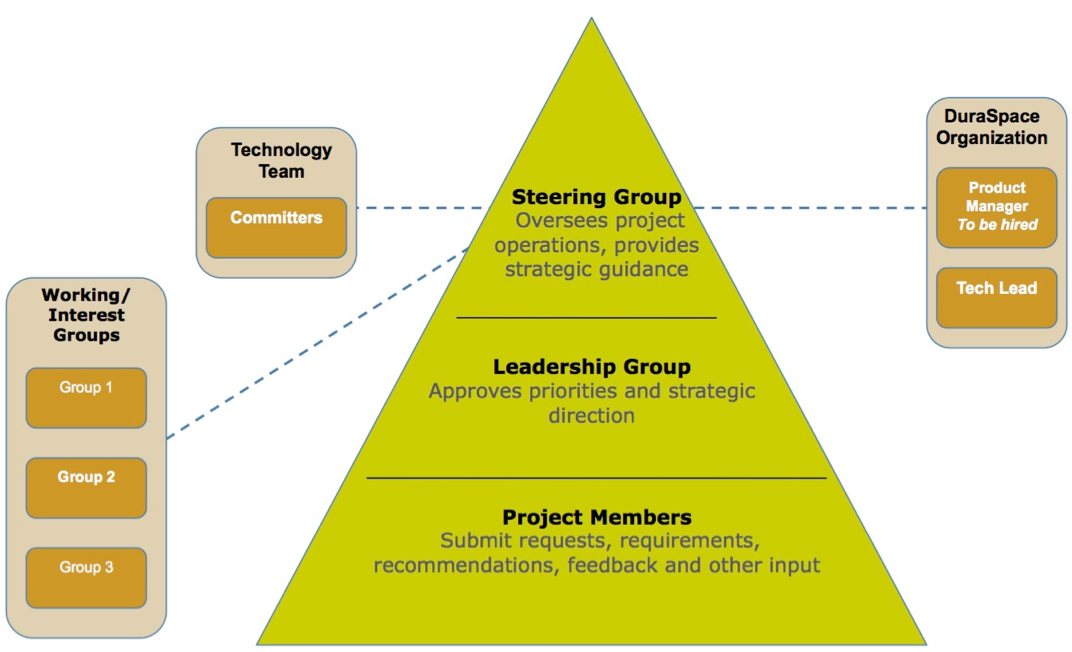
\includegraphics[width=.6\textwidth]{img/DSpace_Project_Governance.png}
\caption{DSpace Governance Model}
\end{figure}

Die DSpace Leadership Group wählt die Steering Group, eine Untergruppe,
die die Sitzungen und Entscheidungen der Leadership Group vorbereitet.
Darüber hinaus gibt es zu einzelnen Themen Working Groups und zu
Bereichen von dauerhaftem Interesse Interest Groups sowie das wichtige
Technology Team. Hier arbeiten die DSpace Committer zusammen, die
gemeinsam für die Pflege des Quellcodes und die Veröffentlichung neuer
Versionen verantwortlich sind. Dies erfolgt in enger Abstimmung mit der
DSpace Leadership Group.

\hypertarget{open-source-finanzieren}{%
\subsection{Open Source finanzieren}\label{open-source-finanzieren}}

Für eine einzelne Einrichtung in Deutschland ist die dauerhafte
Finanzierung einer Mitgliedschaft eine Herausforderung. Anders als bei
lokalen Erweiterungen ist der Mehrwert dem Mittelgeber nicht immer
vermittelbar, knappe Haushaltsbudgets legen andere Prioriäten nah und
Projektmittel stehen für dauerhafte Finanzierungen nicht zur Verfügung.
So sind in der Dura\-Space-Registry (Stand Oktober 2019) 43
DSpace-Installationen in Deutschland eingetragen\footnote{DSpace-Installationen
  in Deutschland siehe
  \url{https://duraspace.org/registry/?gv/_search=\&filter/_10=DSpace\&filter/_4/_6=Germany\&filter/_3=\&filter/_20=\&filter/_28=\&mode=all}.},
aber bis zur Gründung des deutschen DSpace-Konsortiums 2018 gab es keine
deutsche Einrichtung, die Mitglied bei DSpace war. Nur die SUB Göttingen
war bereits Mitglied von DuraSpace, ordnete ihre Mittel aber DuraSpace
in der Gesamtheit der Projekte zu.

Das Konzept, dass die DSpace-Software kostenlos für jeden zur Verfügung
steht, der Erhalt dieses Modells, die Infrastruktur und das Personal für
die Koordination der Entwicklung von Software und Community freiwillig
finanziert werden müssen, ist jedoch erklärungsbedürftig. Hinzu kommt,
dass die gemeinsam finanzierte Infrastruktur Voraussetzung für eine
Weiterentwicklung von DSpace ist, selbst jedoch noch keine neue
Funktionen entwickelt. Für Hosting, Weiterentwicklungen und
institutionelle Anpassungen müssen daher entweder lokale
Programmierkapazitäten aufgebaut werden oder Mittel für Serviceprovider
und eigene Kapazitäten für deren Beauftragung eingeplant werden. Die
Programmierung für DSpace erfolgt fast ausschließlich durch
Programmierer\_innen (\emph{Code Contributors}), die entweder in
Institutionen angestellt sind, die DSpace selbst nutzen, oder bei einem
(registrierten) Serviceprovider für DSpace beschäftigt sind.

Open Access und Open Science sind in den letzten Jahren zu strategischen
Feldern für Bibliotheken geworden. Damit einher geht, dass Bibliotheken
das Umfeld für ihre Aktivitäten selber aktiver gestalten wollen. Es ist
auch ein Bewusstsein dafür gewachsen, welchen Wert Strukturen haben, die
unabhängig von einzelnen Firmen sind und Vendor Lock-Ins verhindern. Es
wird zunehmend bekannter, dass Open Source zwar frei, deshalb aber nicht
kostenlos ist und sich ein unter anderem finanzieller Einsatz für ein
nachhaltiges Open-Source-Modell letztlich rechnet. Das sind einige der
Gründe, die für eine gemeinsame Finanzierung einer Open Source Community
sprechen, wie DSpace es ist.

\hypertarget{das-dspace-konsortium-deutschland}{%
\section{\texorpdfstring{Das \enquote{DSpace-Konsortium
Deutschland}}{Das ``DSpace-Konsortium Deutschland''}}\label{das-dspace-konsortium-deutschland}}

\hypertarget{entstehungsgeschichte-und-beweggruxfcnde}{%
\subsection{Entstehungsgeschichte und
Beweggründe}\label{entstehungsgeschichte-und-beweggruxfcnde}}

Für viele wissenschaftliche Einrichtungen ist DSpace ein wichtiger
Baustein der institutionellen Open-Science-Infrastruktur für Open Access
und Open Data sowie zunehmend auch für Forschungsinformation und eigene
Verlagsangebote. Dies ließ sich unter anderem auf den jährlichen
deutschen Anwendertreffen beobachten, auf denen nicht nur
Weiterentwicklungen präsentiert wurden sondern auch neue, auf
dauerhaften Einsatz angelegte Projekte wie \emph{FIS Universität
Bamberg}, \emph{Göttingen Research Online}, \emph{TUHH Open Research}
oder \emph{DepositOnce -- TU Berlin}.

Dadurch wurde immer deutlicher, dass für die meisten Institutionen
DSpace von strategischer Relevanz ist und sie somit ein intrinsisches
Interesse haben, die Weiterentwicklung langfristig zu sichern und auf
sie Einfluss nehmen zu können. Gleichzeitig ließ die aktive Beteiligung
an den Anwendertreffen auf ein erweitertes Kooperationsinteresse
schließen: 2014 wurde das \enquote{German DSpace User Group Meeting} von
der Universitätsbibliothek der Technischen Universität Berlin (TU
Berlin) ins Leben gerufen. Es war nach mehreren Jahren Pause das erste
Treffen für Nutzer\_innen von DSpace im deutschsprachigen Raum. Seit der
Wiederbelebung durch die TU Berlin hat das Treffen jedes Jahr an
wechselnden Orten stattgefunden, zuletzt im April 2019 an der
Universität Bamberg. Jedes Jahr wuchs die Zahl der Teilnehmer\_innen,
zuletzt auf über 100 Personen.

Wie also können deutsche Institutionen Einfluss nehmen und Teil der
DSpace Governance werden? Die Höhe der Mitgliedsbeiträge für DuraSpace
war an US-amerikanischen Universitäten ausgerichtet, die für
Stiftungsmodelle hohe Summen bereitstellen können. So fallen für eine
Gold-Mitgliedschaft, die einen Sitz in der DSpace Leadership Group
garantiert, 10.000 USD pro Jahr an. Sehr viel Geld für eine einzelne
wissenschaftliche Einrichtung in Deutschland, aber im Rahmen des
Möglichen für eine gemeinsame Finanzierung. Die Universitätsbibliothek
der TU Berlin hat deswegen 2016 die Initiative zur Gründung eines
deutschen Konsortiums ergriffen, um eine gemeinsame, stimmberechtigte
Mitgliedschaft bei DuraSpace zu finanzieren.

Über zwei Jahre lang wurde das Konsortium vorbereitet. In dieser Zeit
wurden gemeinsam mit DuraSpace zwei weitere Mitgliedsstufen entwickelt,
zur Vermeidung des Risikos von Währungskursschwankungen die Zahlung des
Mitgliedsbeitrags in Euro vereinbart und das Modell eines nationalen
Konsortiums ausgearbeitet. Das Konsortium vertritt dabei alle Mitglieder
gemeinsam mit einer Stimme, dafür werden die Beiträge des Konsortiums in
Bezug auf die Vertretung in der Project Governance so gewertet, als
kämen sie von einem Einzelmitglied. Die Rechnung wird von DuraSpace an
die TU Berlin als Konsortialführerin gestellt. Die TU stellt wiederum
Einzelrechnungen an die Mitglieder aus. Damit muss sich nur die TU
Berlin um den Geldtransfer in die USA kümmern, die einzelnen Mitglieder
überweisen ihren Beitrag an die TU Berlin. Eine große Herausforderung
war die steuerrechtliche Klärung der Frage, ob die TU Berlin
Umsatzsteuer auf die Mitgliedsbeiträge erheben und abführen muss.
Hierfür wurde eine spezialisierte Steuerkanzlei von der TU Berlin
beauftragt: Der non-for-profit Status von DuraSpace war für die
Bewertung nicht relevant. Entscheidend war, dass neben dem Stimmrecht
keine weitere Gegenleistung von DuraSpace vereinbart wurde. Damit fallen
keine steuerbaren Leistungen und somit keine Umsatzsteuer an. Die TU
Berlin hat sich außerdem bereit erklärt, die Rechnungsabwicklung
dauerhaft und unentgeltlich zu übernehmen. Damit wurde sichergestellt,
dass alle Mitgliedsbeiträge des Konsortiums komplett der Entwicklung von
DSpace zu Gute kommen.

So konnte der Vertrag mit DuraSpace (der inzwischen auf Lyrasis
überführt wurde) geschlossen und eine Beitrittserklärung für die
Mitglieder entworfen werden. Am 28. Mai 2018 waren alle Fragen von der
TU Berlin geklärt und Jürgen Christof, Leitender Bibliotheksdirektor der
Universitätsbibliothek der TU Berlin, informierte die Direktionen der
deutschen Einrichtungen mit DSpace-Installationen über das geplante
Konsortium und lud zu einer Informationsveranstaltung auf dem 107.
Bibliothekartag am 13. Juni 2018 ein.

\hypertarget{ziele-des-konsortium}{%
\subsection{Ziele des Konsortium}\label{ziele-des-konsortium}}

Durch den offenen Ansatz, dem sich die Community verschrieben hat,
verspricht DSpace Nachhaltigkeit für Repositorien und damit für
Forschungsinfrastrukturen. Das \enquote{DSpace-Konsortium Deutschland}
trat mit dem Ziel an, einen regelmäßigen, jährlichen, finanziellen
Beitrag zu DSpace zu leisten und damit die Verfügbarkeit von
Open-Source-Software für Repositorien zu sichern. Das Konsortium
erleichtert es Institutionen in Deutschland, finanzielle Beiträge zu
DSpace zu leisten, indem die steuerrechtlichen Prüfungen und die
Vertragsausgestaltung durch die TU Berlin für alle Mitglieder übernommen
wurde.

Über die Mitgliedsbeiträge sollte mindestens eine Gold-Mitgliedschaft
finanziert werden, die dem Konsortium einen Platz in der DSpace
Leadership Group sichert, ohne auf Wahlen unter den DSpace-Mitgliedern
angewiesen zu sein. Damit sollte strategischer Einfluss auf DSpace
gesichert und die Interessen deutscher DSpace-Nutzer\_innen in der
Project Governance vertreten werden.

\hypertarget{ergebnisse}{%
\subsection{Ergebnisse}\label{ergebnisse}}

Die Gründung des \enquote{DSpace-Konsortium Deutschland} unter Führung
der TU Berlin war sehr erfolgreich. Zum 1. Juli 2018 startet das
DSpace-Konsortium Deutschland mit 25 institutionellen Mitgliedern. Ein
halbes Jahr später traten drei weitere Mitglieder bei.

Die Mitgliedsbeiträge übertrafen bereits im Gründungs- und auch im
Folgejahr alle Erwartungen und ermöglichen es, einen signifikanten
Beitrag zur DSpace Community zu leisten. In der DSpace Leadership Group
wird das Konsortium von Beate Rajski, der Sprecherin des Konsortiums,
vertreten. Der zweite Sprecher des Konsortiums Pascal Becker wurde
darüber hinaus von The Library Code GmbH, einem DSpace Service Provider,
in die DSpace Leadership Group entsandt und auch in die DSpace Steering
Group gewählt, so dass auch er das Konsortium in der Project Governance
vertreten kann.

Durch die Mitarbeit in den Gremien der DSpace Governance wurden die
Interessen der europäischen und deutschen Mitglieder innerhalb der
DSpace Community sichtbarer. So geht die Gründung einer DSpace Working
Group zum Thema Datenschutzgrundverordnung (DSGVO) auf das
DSpace-Konsortium Deutschland zurück. Das Konsortium hat sich auch in
die Gespräche vor der Fusion von DuraSpace und Lyrasis eingebracht und
Anteil daran, dass die Interessen internationaler DSpace-Mitglieder bei
der Fusion der beiden US-amerikanischen Organisationen berücksichtigt
wurden. Es hat sich in diesem Sinn im Vorfeld der Fusion erfolgreich für
die Vereinbarung eines Memorandum of Understanding zwischen DuraSpace,
Lyrasis und der DSpace Community eingesetzt.

Und letztlich sorgt das Konsortium mit seinen beiden Sprecher\_innen für
einen besseren Informationsfluss aus der DSpace Community hin zu seinen
Mitgliedern und zurück in die Community.

\hypertarget{kommunikation-und-information}{%
\subsection{Kommunikation und
Information}\label{kommunikation-und-information}}

Das DSpace-Konsortium Deutschland trifft sich einmal im Jahr im Rahmen
des DSpace Anwendertreffens zu einer nichtöffentlichen Sitzung. An
diesem speziellen Teil des Anwendertreffens sind nur Vertreter\_innen
der Mitglieder teilnahmeberechtigt. Dort werden die Sprecher\_innen des
Konsortiums für das nächste Jahr gewählt, es gibt Zeit für Fragen der
Mitglieder und es kann über Arbeitsweise und Aktivitäten des Konsortiums
diskutiert werden. Für die Kommunikation zwischen den Treffen und den
Informationsfluss aus der DSpace Leadership Group gibt es eine
Mailingliste für die Mitglieder des Konsortiums. Über die Mailingliste
informieren die Sprecher\_innen des Konsortiums regelmäßig zu den
Treffen der Project Governance und zu sonstigen Entwicklungen innerhalb
der DSpace Community. Die Mailingliste ermöglicht es auch jedem Mitglied
von sich aus Themen in das Konsortium zu tragen. Im DSpace-Wiki pflegt
das Konsortium eine Seite, auf der alle Verträge einsehbar sind, alle
Mitglieder aufgelistet werden und auf der auch die Beitrittserklärung
für neue Mitglieder gefunden werden kann:
\url{https://wiki.duraspace.org/display/DSPACE/DSpace-Konsortium+Deutschland}.

\hypertarget{warum-institutionen-sich-im-dspace-konsortium-engagieren-sollten}{%
\subsection{Warum Institutionen sich im DSpace-Konsortium engagieren
sollten}\label{warum-institutionen-sich-im-dspace-konsortium-engagieren-sollten}}

\enquote{Kommerzielle Akteure schicken sich an, ein ganzes
Betriebssystem inklusive integrierter Werkzeuge zu schaffen, das
unablässig Verhalten von Wissenschaftlern und Performanz von
Wissenschaft protokolliert.} schrieb Ulrich Herb 2018.\footnote{Herb, U.
  (2018). Zwangsehen und Bastarde : Wohin steuert Big Data die
  Wissenschaft? In: Information -- Wissenschaft \& Praxis, 69(2-3), S.
  81-88. \url{https://doi.org/10.1515/iwp-2018-0021}, S. 81.}

Erinnert sei zum Beispiel an die Übernahme des maßgeblichen Open Access
Repositories im Bereich der Sozial- und Geisteswissenschaften Social
Science Research Network (SSRN) durch Elsevier im Mai 2016.\footnote{Siehe
  \url{https://www.elsevier.com/connect/ssrn-the-leading-social-science-and-humanities-repository-and-online-community-joins-elsevier}.}

Das DSpace-Konsortium Deutschland hilft dabei, im internationalen Markt
der Repositoriensoftware ein Angebot zu erhalten und weiterzuentwickeln,
das frei von Vendor Lock-Ins ist und dem Aufbau neuer Abhängigkeiten im
Bereich wissenschaftlicher Publikations- und
Forschungsdateninfrastruktur entgegen steht.

DSpace steht als Open-Source-Software zur Nutzung frei zur Verfügung.
Dass auch das finanzielle Engagement "frei"willig ist, sollte über
dessen Notwendigkeit nicht hinwegtäuschen. Letztlich liegt es im
Interesse der Institutionen, die DSpace nutzen, dafür zu sorgen, dass
das Modell der freiwilligen Beiträge sich trägt und der
softwaretechnische Kern von Open-Access- und
Forschungsdateninfrastrukturen nachhaltig betreibbar bleibt.

Mit dem deutschen DSpace-Konsortium steht Institutionen, die in
Deutschland DSpace einsetzen, egal ob groß, mittel oder klein, die
Möglichkeit offen, gemeinsam mit einer starken Stimme und finanziellem
Engagement zum Erfolg von DSpace beizutragen und Erhalt und
Weiterentwicklung nachhaltiger und herstellerunabhängiger Strukturen zu
sichern.

\hypertarget{mitglieder-im-dspace-konsortium-deutschland-stand-oktober-2019}{%
\subsection{Mitglieder im DSpace-Konsortium Deutschland (Stand: Oktober
2019)}\label{mitglieder-im-dspace-konsortium-deutschland-stand-oktober-2019}}

\begin{itemize}
\item
  Bergische Universität Wuppertal
\item
  Bundesanstalt für Wasserbau
\item
  Bundesinstitut für Berufsbildung (BIBB)
\item
  Deutsches Institut für Urbanistik gGmbH
\item
  Direktion IZUS / Universitätsbibliothek Stuttgart
\item
  Eberhard Karls Universität Tübingen
\item
  Heinrich-Heine-Universität Düsseldorf
\item
  Humboldt-Universität zu Berlin
\item
  kiz / Kommunikations- und Informationszentrum der Universität Ulm
\item
  Leibniz-Zentrum für Psychologische Information und Dokumentation
  (ZPID)
\item
  Martin-Luther-Universitätbibliothek Halle-Wittenberg
\item
  Medizinische Bibliothek der Charité
\item
  Schloss Dagstuhl -- Leibniz-Zentrum für Informatik GmbH
\item
  Staats- und Universitätsbibliothek Hamburg - Carl von Ossietzky
\item
  Technische Universität Berlin
\item
  TU Dortmund Kreditorenbuchhaltung
\item
  Universität Konstanz
\item
  Universität Siegen
\item
  Universitäts- und Landesbibliothek Bonn
\item
  Universitäts- und Landesbibliothek Darmstadt
\item
  Universitätsbibliothek Bamberg
\item
  Universitätsbibliothek der Freien Universität Berlin
\item
  Universitätsbibliothek Kassel
\item
  Universitätsbibliothek Mainz
\item
  Universitätsbibliothek Osnabrück
\item
  Universitätsbibliothek TUHH
\item
  Universitätsbibliothek Vechta
\item
  ZBW -- Leibniz-Informationszentrum Wirtschaft
\end{itemize}

%autor
\begin{center}\rule{0.5\linewidth}{\linethickness}\end{center}

\textbf{Beate Rajski} ist Bibliothekarin und arbeitet seit 30(!) Jahren
an der TU Hamburg. Sie ist Fachreferentin für Forschungsdaten und
Abteilungsleiterin der Digitalen Dienste der Universitätsbibliothek.
2018 bis 2020 leitet sie das Projekt Forschungsdatenmanagement für
Hamburg Open Science, ein Programm, in dem DSpace sowohl für
Open-Access- und Forschungsdatenrepositorien als auch für FIS-Funktionen
zum Einsatz kommt. Die Idee des DSpace-Konsortiums hat sie von Anfang an
unterstützt und ist seit der Gründung Sprecherin und Mitglied der DSpace
Leadership Group.

\textbf{Pascal Becker} hatte die Idee, ein nationales DSpace-Konsortiums
zu gründen und hat diese Idee seit 2016 verfolgt. Er hat Informatik
studiert und arbeitet seit über 13 Jahren in bibliothekarischen
Umgebungen und an Open-Access-Repositorien, zuletzt an der TU Berlin. Er
ist Geschäftsführer des von ihm gegründeten DSpace Service Provider The
Library Code GmbH (\url{https://www.the-library-code.de/}), zweiter
Sprecher des DSpace-Konsortiums Deutschland, organisiert seit 2014
jährlich das DSpace Anwendertreffen, ist Mitglied in der DSpace
Committer, DSpace Leadership, DSpace Steering Group und in der DataCite
Services and Technology Steering Group.

\end{document}
